\clearpage
\item \points{20} {\bf A Simple Neural Network}

Let $X = \{x^{(1)}, \cdots, x^{(m)}\}$ be a dataset of $m$ samples with 2 features, i.e $x^{(i)} \in \mathbb{R}^2$. The samples are classified into 2 categories with labels $ y^{(i)} \in \{0, 1\}$. A scatter plot of the dataset is shown in Figure $\ref{fig:nn_plot}$:
	\begin{figure}[htbp] 
		\centering
		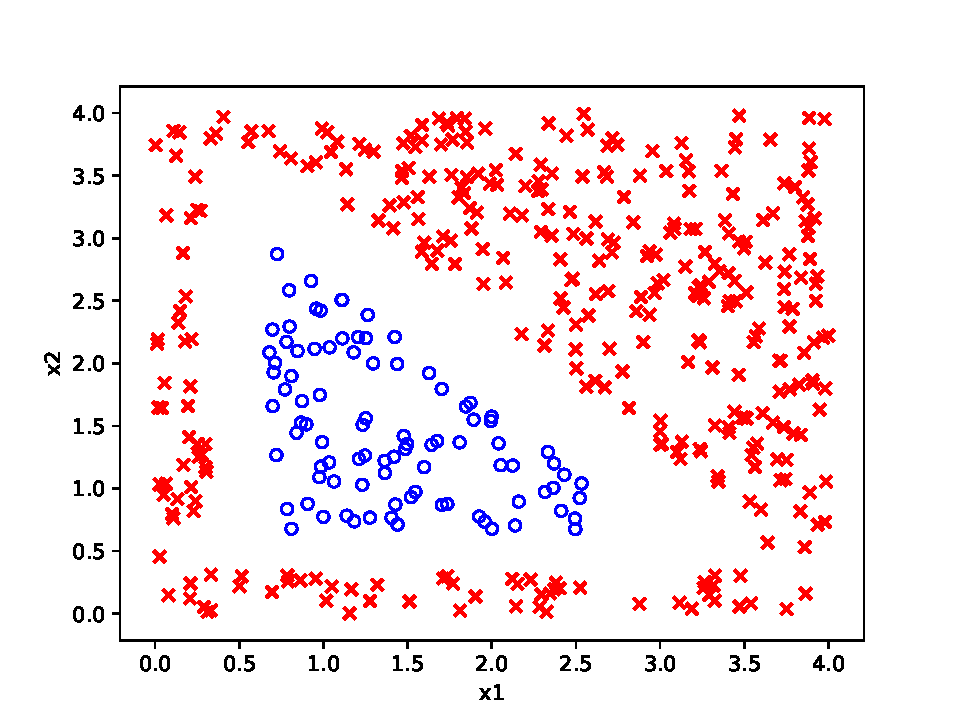
\includegraphics[scale=0.5]{../data/nn_plot.pdf}
		\caption{Plot of dataset $X$.}
		\label{fig:nn_plot}
	\end{figure}

	The examples in class $1$ are marked as as ``$\times$" and examples in class $0$ are marked as ``$\circ$". We want to perform binary classification using a simple neural network with the architecture shown in Figure $\ref{fig:nn_arc}$:
	\begin{figure}[htbp]
		\centering
		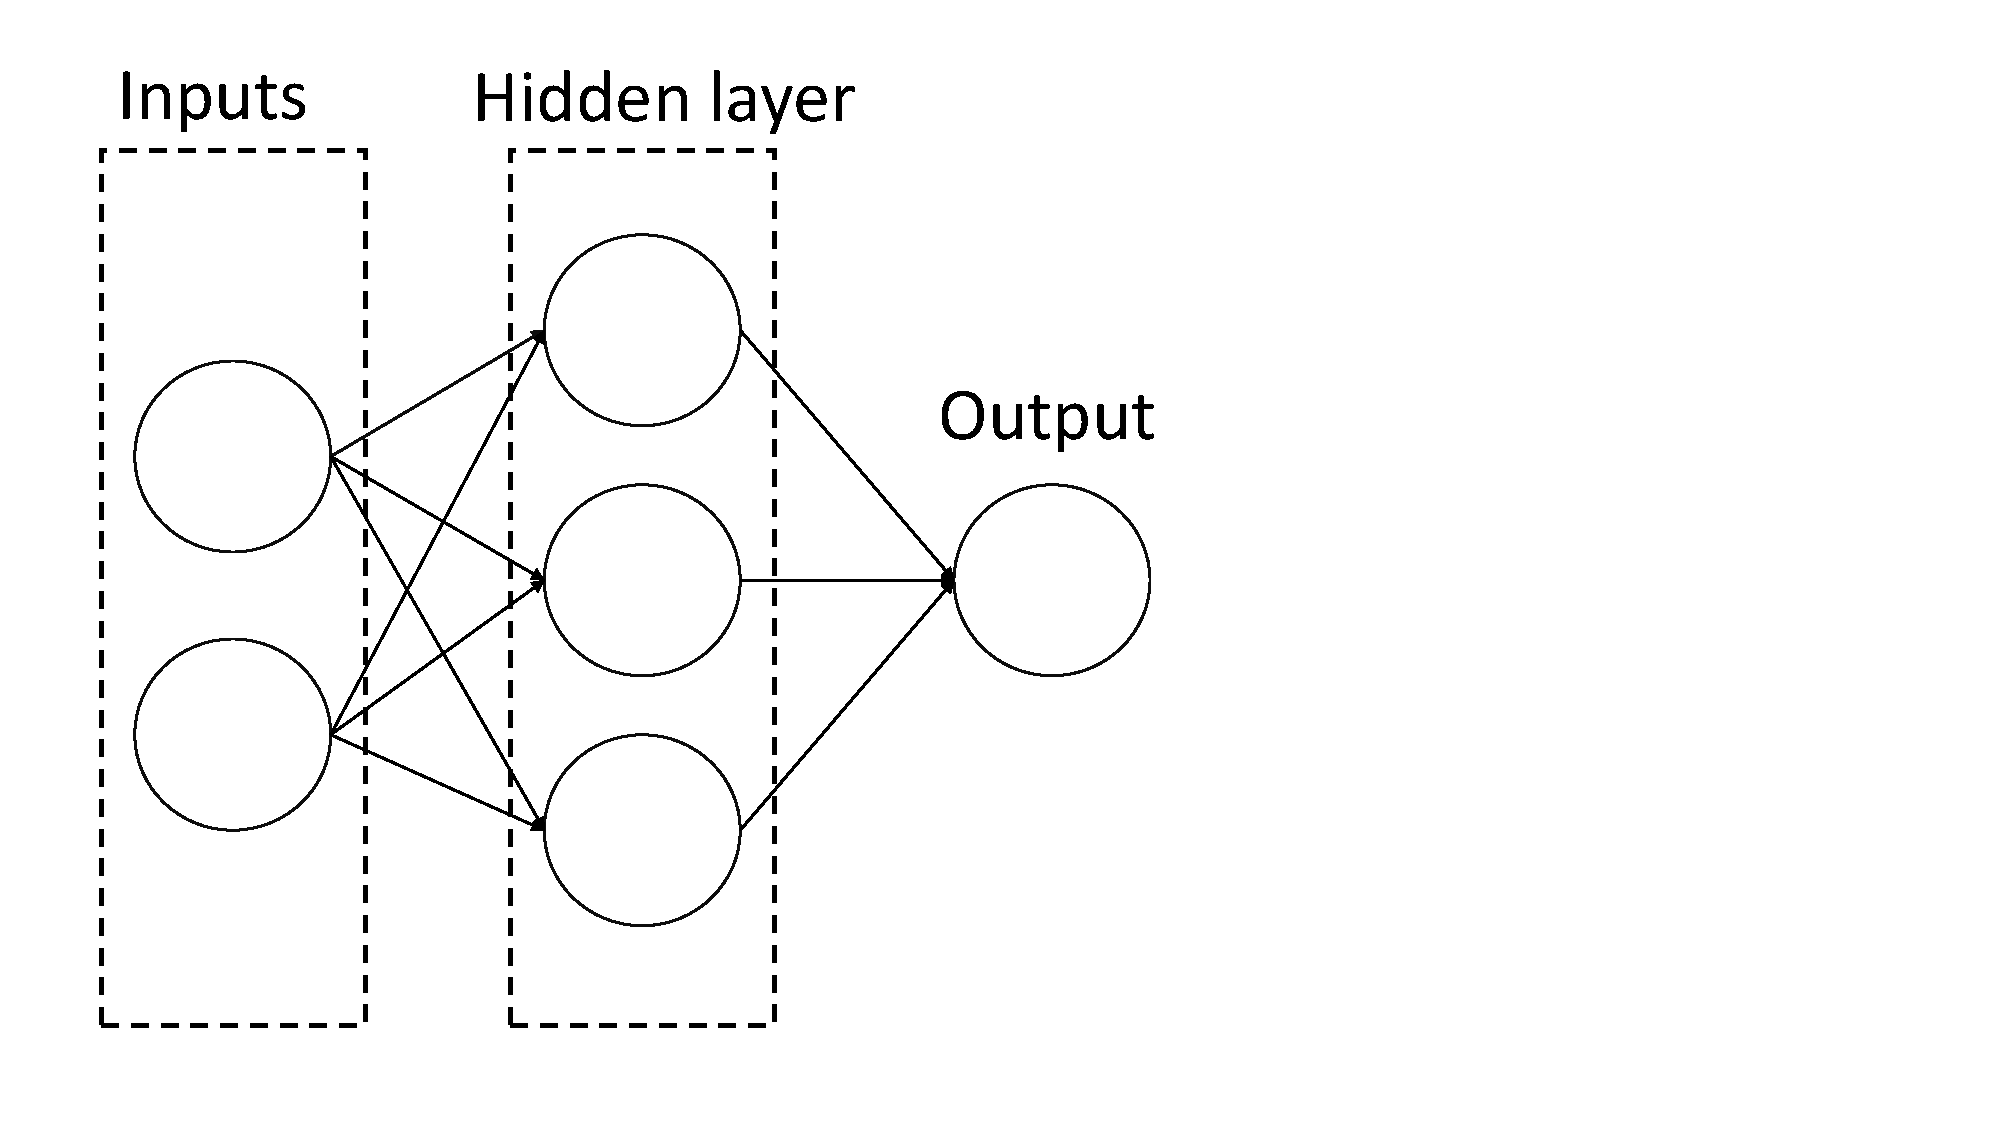
\includegraphics[scale=0.2, trim = 0 0 360 0, clip]{../data/nn_architecture.pdf}
		\caption{Architecture for our simple neural network.}
		 \label{fig:nn_arc}
	\end{figure}

	Denote the two features $x_1$ and $x_2$, the three neurons in the hidden layer $h_1, h_2$, and $h_3$, and the output neuron as $o$. Let the weight from $x_i$ to $h_j$ be $w_{i, j}^{[1]}$ for $i \in \{1, 2\}, j \in \{1, 2, 3\}$, and the weight from $h_j$ to $o$ be $w_{j}^{[2]}$. Finally, denote the intercept weight for $h_j$ as $w_{0, j}^{[1]}$, and the intercept weight for $o$ as $w_{0}^{[2]}$. For the loss function, we'll use average squared loss instead of the usual negative log-likelihood:
  $$l = \frac{1}{m}\sum_{i=1}^{m}(o^{(i)} - y^{(i)})^2,$$
  where $o^{(i)}$ is the result of the output neuron for example $i$.

\begin{enumerate}

  \item \subquestionpoints{5} Suppose we use the sigmoid function as the activation function for $h_1, h_2, h_3$ and $o$.
      What is the gradient descent update to $w_{1, 2}^{[1]}$, assuming we use a learning rate of $\alpha$?
      Your answer should be written in terms of $x^{(i)}$, $o^{(i)}$, $y^{(i)}$, and the weights.\\
      
\ifnum\solutions=1 {
  \begin{answer}
 Recall $\sigma$ denotes the sigmoid function and for computations $\sigma' = \sigma (1 - \sigma)$ is handy.
 Write $h_i = \sigma(\omega _{1,i}^{[1]}x_1 + \omega _{2,i}^{[1]}x_2 + b_j^{[1]}) (1)$ for $j = 1,2 ,3$ and $o = \sigma(\omega _{1}^{[2]}h_1 + \omega _{2}^{[2]}h_2 + b^{[2]})$
The graduate descent update for $\omega _{1,2}^{[1]}$ is
$$\omega _{1,2}^{[1]} = \omega _{1,2}^{[1]} - \alpha \frac{\partial l}{\partial \omega _{1,2}^{[1]}}.$$
Now we  will evaluate the partial derivate using the chain rule and by noting that in order to evaluate the desired partial
derivative we only need to look at the function $h_2.$

$$\frac{\partial l}{\partial \omega _{1,2}^{[1]}}= \frac 2m\sum_{i}(o^{(i)} - y^{(i)})\frac{\partial o^{(i)}}{\partial \omega _{1,2}^{[1]}}$$
$$ = \frac 2m\sum_{i}(o^{(i)} - y^{(i)}) o^{(i)}(1 - o^{(i)})\omega_2^{[2]}h_2(1 - h_2)x^{(i)}.$$ 

Although, the final outcome is expressed in terms of the function $h_2$ one can easily replace it with using (1) and putting the superscript $(i).$      
 \end{answer}

} \fi


  \ifnum\solutions=1 {
  \clearpage
} \fi
\item \subquestionpoints{10} Now, suppose instead of using the sigmoid function for the activation function
      for $h_1, h_2, h_3$ and $o$,
      we instead used the step function $f(x)$, defined as
		\begin{align*}
		f(x) = \begin{cases}
		1, x \ge 0 \\
		0, x < 0
		\end{cases}
		\end{align*}

Is it possible to have a set of weights that allow the neural network to classify this dataset with 100\% accuracy?

If it is possible, please provide a set of weights that enable 100\% accuracy by completing \texttt{optimal\_step\_weights} within \texttt{src/p01\_nn.py} and explain your reasoning for those weights in your PDF.

If it is not possible, please explain your reasoning in your PDF. (There is no need to modify \texttt{optimal\_step\_weights} if it is not possible.)


\textbf{Hint:} There are three sides to a triangle, and there are three neurons in the hidden layer.

\ifnum\solutions=1 {
  \begin{answer}
  Yes, it is possible. If we look at the picture of the dataset we, can see that all the 'o' labels are within the intersection of the lines(which forms a triangle)
 
Let $A$ be a boolean given by $A = (x_1 > 0.5) \& (x_2 > 0.5))\& (x_1 + x_2 < 4).$
We want to choose the weights and the biases such that $A = 1$ if and only if $o = 1.$
If we set $h _1 = f(2x_1 - 1),\ \ h_2 = f(2x_2 - 1),\ \  h_3 = f(-x_1 - x_2 + 4)$ (by choosing the weights and biases accordingly)
we see that $A = 1$ implies that $h_1 = 1 \& h_2 = 1 \& h_3 = 1$ and $A = 0$ implies that $h_1h_2h_3 = 0.$
Now we set $o = f(2h_1 + 2h_2 + 2h_3 - 5).$ Now if $A = 1$, then $h_1 = h_2 = h_3 = 1$ and hence $o = 1.$
If $A = 0$ then since at least one of the $h_i's$ is 0  one has $2h_1 + 2h_2 + 2h_3 - 5 < 0$ and so $o = 0.$ 


 \end{answer}

} \fi

  
  \ifnum\solutions=1 {
  \clearpage
} \fi
\item \subquestionpoints{10} Let the activation functions for $h_1, h_2, h_3$ be the linear function $f(x) = x$ and the activation function for $o$ be the same step function as before.

Is it possible to have a set of weights that allow the neural network to classify this dataset with 100\% accuracy?

If it is possible, please provide a set of weights that enable 100\% accuracy by completing \texttt{optimal\_linear\_weights} within \texttt{src/p01\_nn.py} and explain your reasoning for those weights in your PDF.

If it is not possible, please explain your reasoning in your PDF. (There is no need to modify \texttt{optimal\_linear\_weights} if it is not possible.)


\ifnum\solutions=1 {
  \begin{answer}
Not possible.
    If the function is linear then as the composition of linear functions is also linear then it would follow that $o$ can be written as
    $o = a_1x_1 + a_2x_2 + b$ for some parameters $a_1,a_2.b.$ Since this represents a single line, it is not possible
    for this line to separate the positive and negative examples.
    
\end{answer}

} \fi


\end{enumerate}
